\section{Results}\label{sec:results}

\subsection{The naive protocol selects a degenerate operating point}\label{sec:broken}

On an initial sweep over $\ell \in \{10, 12, 14, 16\}$ and $\alpha \in \{4, 8, 12\}$, validation MC2 alone selects $\ell{=}\NaiveLayer$, $\alpha{=}\NaiveAlpha$. The injected vector is then \NaiveNormRatio$\times$ the median residual norm at that layer, held-out perplexity is \NaivePplRatio$\times$ baseline, and free generation degenerates into repetitive token fragments (Appendix~\ref{app:generations}).
\newpage
Despite this collapse, teacher-forced MC2 nominally improves by \NaiveDecDelta{} \NaiveDecDeltaCI{}. MC1 moves by \NaiveDecDeltaMcOne{} \NaiveDecDeltaMcOneCI{} from a baseline of \BaseMcOne. Teacher forcing conditions each answer token on the reference text rather than the model's continuation, so it can reward a perturbation that cannot generate coherent language.

The depth statistic is also uninterpretable at this point. The full condition matrix gives $\rho(\text{aligned-64}) = \NaiveRhoAlSixtyFour$, with random-projection controls also near $1$, but the denominator $\Delta(v)$ is statistically zero. The bootstrap interval \NaiveRhoAlSixtyFourCI{} reflects a ratio of two noisy estimates rather than evidence for a downstream effect. Both preconditions in Section~\ref{sec:method} therefore fail. All subsequent results use the coherence-gated operating points from Section~\ref{sec:setup} and locate an effect only after establishing that it is usable.

\begin{table}[h]
\centering
\small
\setlength{\tabcolsep}{16pt}
\renewcommand{\arraystretch}{1.15}
\begin{tabular}{lccc}
\toprule
condition & MC2 & $\Delta$MC2 & $\rho$ \\
\midrule
\multicolumn{4}{l}{\emph{CAA} \quad ($\ell^{*}{=}\DecLayer$, $\alpha^{*}{=}\DecAlpha$, PPL ratio \DecPplRatio)} \\
\midrule
$v_{\mathrm{dec}}$ & $0.436$ & $-0.035$ & n/a \\
$v^{\perp}$ al-16 & $0.426$ & $-0.045$ & $1.30$ \,{\scriptsize $[-0.12,\, 3.16]$} \\
$v^{\perp}$ al-64 & $0.429$ & $-0.042$ & $1.20$ \,{\scriptsize $[0.01,\, 2.99]$} \\
$v^{\perp}$ al-256 & $0.424$ & $-0.047$ & $1.35$ \,{\scriptsize $[-1.10,\, 4.46]$} \\
$v^{\perp}$ al-1024 & $0.424$ & $-0.047$ & $1.35$ \,{\scriptsize $[-1.70,\, 5.99]$} \\
$v^{\perp}$ cur & $0.437$ & $-0.034$ & $0.97$ \,{\scriptsize $[0.63,\, 1.25]$} \\
$v^{\perp}$ stat & $0.436$ & $-0.035$ & $1.01$ \,{\scriptsize $[0.75,\, 1.37]$} \\
$v^{\parallel}$ al-64 & $0.481$ & $+0.010$ & $-0.30$ \,{\scriptsize $[-2.63,\, 0.67]$} \\
$v^{\perp}$ al-64 nm & $0.427$ & $-0.044$ & $1.26$ \,{\scriptsize $[0.19,\, 3.19]$} \\
rand s0 & $0.432$ & $-0.039$ & $1.13$ \,{\scriptsize $[0.58,\, 1.95]$} \\
rand s1 & $0.440$ & $-0.031$ & $0.89$ \,{\scriptsize $[0.23,\, 1.37]$} \\
rand s2 & $0.438$ & $-0.033$ & $0.94$ \,{\scriptsize $[0.57,\, 1.22]$} \\
\midrule
\multicolumn{4}{l}{\emph{mass-mean} \quad ($\ell^{*}{=}\MmLayer$, $\alpha^{*}{=}\MmAlpha$, PPL ratio \MmPplRatio)} \\
\midrule
$v_{\mathrm{dec}}$ & $0.543$ & $+0.073$ & n/a \\
$v^{\perp}$ al-16 & $0.539$ & $+0.069$ & $0.94$ \,{\scriptsize $[0.81,\, 1.07]$} \\
$v^{\perp}$ al-64 & $0.540$ & $+0.069$ & $0.95$ \,{\scriptsize $[0.79,\, 1.14]$} \\
$v^{\perp}$ al-256 & $0.543$ & $+0.072$ & $0.99$ \,{\scriptsize $[0.80,\, 1.27]$} \\
$v^{\perp}$ al-1024 & $0.564$ & $+0.093$ & $1.28$ \,{\scriptsize $[0.95,\, 2.00]$} \\
$v^{\perp}$ cur & $0.541$ & $+0.071$ & $0.97$ \,{\scriptsize $[0.90,\, 1.04]$} \\
$v^{\perp}$ stat & $0.551$ & $+0.080$ & $1.10$ \,{\scriptsize $[1.04,\, 1.23]$} \\
$v^{\parallel}$ al-64 & $0.502$ & $+0.032$ & $0.43$ \,{\scriptsize $[0.27,\, 0.76]$} \\
$v^{\perp}$ al-64 nm & $0.539$ & $+0.068$ & $0.93$ \,{\scriptsize $[0.78,\, 1.10]$} \\
rand s0 & $0.545$ & $+0.074$ & $1.01$ \,{\scriptsize $[0.96,\, 1.08]$} \\
rand s1 & $0.549$ & $+0.079$ & $1.08$ \,{\scriptsize $[1.02,\, 1.20]$} \\
rand s2 & $0.541$ & $+0.070$ & $0.96$ \,{\scriptsize $[0.88,\, 1.02]$} \\
\bottomrule
\end{tabular}

\caption{Headline condition matrix on the \NTest{} held-out test questions; the shared unsteered baseline has MC2 $= \BaseMcTwo$. $\rho$ is the fraction of each family's steering effect that survives projection, with paired-bootstrap 95\% intervals. CAA's $\Delta$MC2 interval \DecTestDeltaCI{} contains zero, so its $\rho$ values are shown but not interpreted; percentile ratio intervals are not valid confidence sets when the denominator is not bounded away from zero. The mass-mean interval is bounded away from zero ($\Delta$MC2 \MmTestDelta{} \MmTestDeltaCI). Figure~\ref{fig:forest} shows the paired deltas.}
\label{tab:matrix}
\end{table}

\begin{figure}[t]
\centering
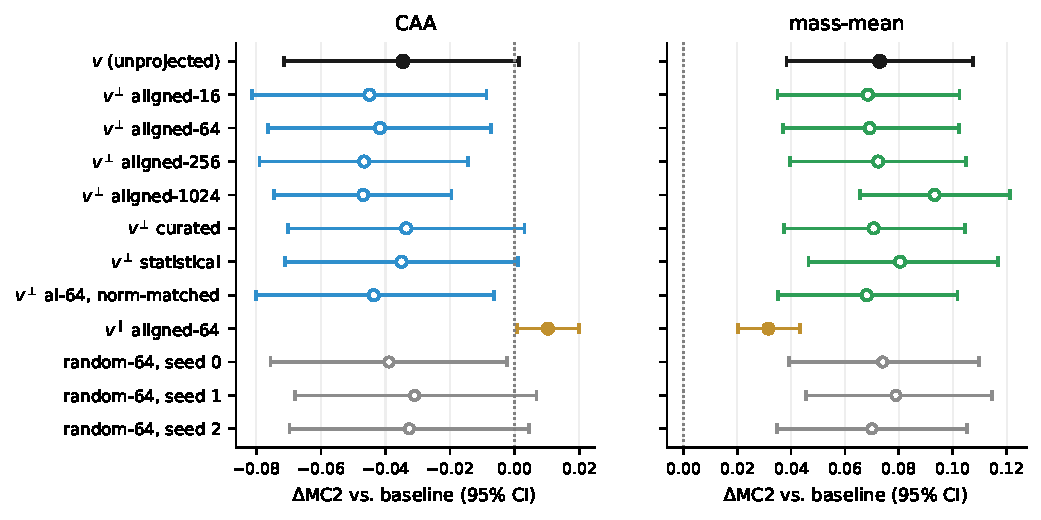
\includegraphics[width=\textwidth]{../figures/forest.pdf}
\caption{Paired per-question $\Delta$MC2 for every condition, with 95\% bootstrap intervals. Left: CAA. The unprojected vector and every orthogonal projection sit at or below zero; only the readout-aligned parallel component (filled triangles) is positive. Right: mass-mean. Every orthogonal projection overlaps the unprojected vector, and the random-64 controls (open diamonds) are indistinguishable from the aligned excisions.}
\label{fig:forest}
\end{figure}
\FloatBarrier

\subsection{Selected CAA point: a large vocabulary shift without a reliable truthfulness gain}\label{sec:caa}

At its best coherent operating point ($\ell^{*}{=}\DecLayer$, $\alpha^{*}{=}\DecAlpha$; perplexity ratio \DecPplRatio; injected norm $\DecNormRatio\times$ the median residual), CAA's validation gain of \DecValDelta{} does not replicate. On the \NTest{} held-out questions, $\Delta$MC2 is \DecTestDelta{} \DecTestDeltaCI{} and $\Delta$MC1 is \DecTestDeltaMcOne{} \DecTestDeltaMcOneCI{} (Figure~\ref{fig:forest}, left). CAA still shifts the curated honest-versus-deceptive logit gap by \DecEtaCurDeltaVdec{} logits at the answer position, but provides no reliable truthfulness gain.

The readout-aligned rank-64 component alone yields $\Delta$MC2 of \DecParDelta, while the certified-orthogonal remainder yields \DecPerpDelta. The parallel component's positive point estimate is consistent with a readout-level contribution, but neither the full vector nor the orthogonal remainder provides a reliable truthfulness gain. Vocabulary movement therefore does not by itself establish useful honesty steering. The selected-point null is not hiding a comparable effect elsewhere in the grid: across all \CaaGridNCoherent{} coherent test-set settings, CAA's largest gain is \CaaGridMaxDelta{} \CaaGridMaxDeltaCI{} (Appendix~\ref{app:caagrid}), less than one fifth of the mass-mean effect. Table~\ref{tab:matrix} reports CAA's $\rho$ values for completeness, but its denominator interval contains zero, so those ratios cannot locate a behavioral effect.

\subsection{Mass-mean improves truthfulness and is predominantly downstream under the tested readout}\label{sec:mm}

Mass-mean improves truthfulness at a coherent operating point. At $\ell^{*}{=}\MmLayer$, $\alpha^{*}{=}\MmAlpha$ (perplexity ratio \MmPplRatio; injected norm $\MmNormRatio\times$ the median residual), test MC2 rises by \MmTestDelta{} \MmTestDeltaCI{} and MC1 by \MmTestDeltaMcOne{} \MmTestDeltaMcOneCI. The full condition matrix appears in Figure~\ref{fig:forest} (right). Figure~\ref{fig:scatter} shows that \MmFracImproving{} of questions improve, so the mean is not driven by a few outliers. The projected and unprojected vectors also have similar per-question patterns, which indicates that excision preserves the original behavioral effect rather than replacing it with a different average gain.

\begin{figure}[t]
\centering
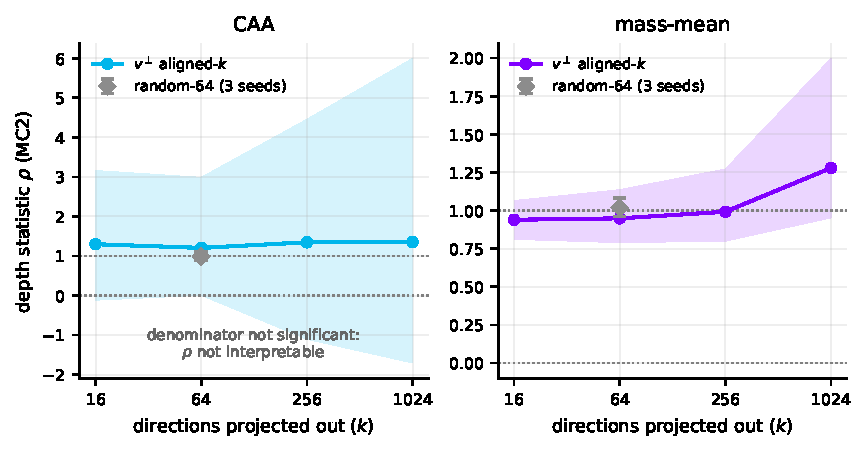
\includegraphics[width=0.95\textwidth]{../figures/rho_curve.pdf}
\caption{Depth statistic $\rho(k)$ after excising the top-$k$ readout-aligned directions (bands: 95\% paired-bootstrap intervals; open diamond: random-64 controls, with the range over three seeds). For mass-mean, $\rho$ stays at or above \MmRhoKMin{} and matches the random controls at $k{=}64$; at $k{=}1024$ the point estimate rises, opposite to the suppression prediction. CAA's interval spans zero at every $k$ because its denominator is not significant.}
\label{fig:rho}
\end{figure}

Projecting out the 64 most readout-aligned directions zeros the calibration-averaged first-order direct contribution to the tokens the vector moves most, with a certified residual of at most \CertWorst{} logits. The behavioral effect remains: $\rho = \MmRhoAlSixtyFour$ \MmRhoAlSixtyFourCI. Random 64-dimensional excisions give $\rho$ between \MmRhoRandMin{} and \MmRhoRandMax, and the paired aligned-minus-random contrast is \MmAlignedMinusRandom{} \MmAlignedMinusRandomCI{}. Removing the aligned contribution is therefore statistically indistinguishable from equal-rank random removal under the three sampled seeds. This comparison isolates readout specificity: random removal controls for generic projection damage, while aligned removal targets the pathway required by suppression. Pure suppression predicts a contrast near $-1$, whereas the interval excludes an aligned-specific cost larger than about one quarter of the effect. The removed parallel component contains 30\% of the vector's norm but produces only \MmParDelta{} $\Delta$MC2 in isolation, less than half the full effect (Figure~\ref{fig:decomp}, left). It is neither necessary nor sufficient for the full gain. The supported conclusion is that most of the effect is downstream under this readout, not that the vocabulary contribution is exactly zero.

The result is stable across projection and outcome definitions. From $k{=}16$ to $k{=}1024$, one quarter of the residual dimension, the point estimate never falls below \MmRhoKMin{} and no interval lower bound falls below \MmRhoKCiFloor; at $k{=}1024$, $\rho = \MmRhoAlBig$ \MmRhoAlBigCI{} (Figure~\ref{fig:rho}). If suppression were distributed across a larger set of aligned tokens, removing more directions should drive $\rho$ toward zero. Instead, the estimates are non-decreasing in $k$, and every interval contains $1$. These intervals do not establish exact invariance, but they show no detectable attenuation as the excised rank grows. The curated and statistical token sets give $\rho = \MmRhoCur$ and $\rho = \MmRhoStat$, with spread $\sigma_T = \MmSigmaT$ across the three constructions. Norm matching gives $\rho = \MmRhoNm$. Using MC1 exact-match accuracy instead gives $\rho = \MmRhoAlSixtyFourMcOne$ \MmRhoAlSixtyFourMcOneCI{} at aligned-64. Agreement across token sets, vector norms, and scoring rules makes the depth finding less dependent on one analysis choice.

On 150 model-paraphrased questions, mass-mean retains a $\Delta$MC2 of \MmOodDeltaVdec{} \MmOodDeltaVdecCI, and the projected vector retains the effect: $\rho_{\mathrm{OOD}} = \MmRhoOod$ \MmRhoOodCI{} (Figure~\ref{fig:decomp}, right). The paraphrase comparison tests whether both the gain and its depth depend on the original wording. Their persistence makes a prompt-specific lexical shortcut less plausible, although the evidence is limited to model-generated paraphrases of the same benchmark.

\begin{figure}[t]
\centering
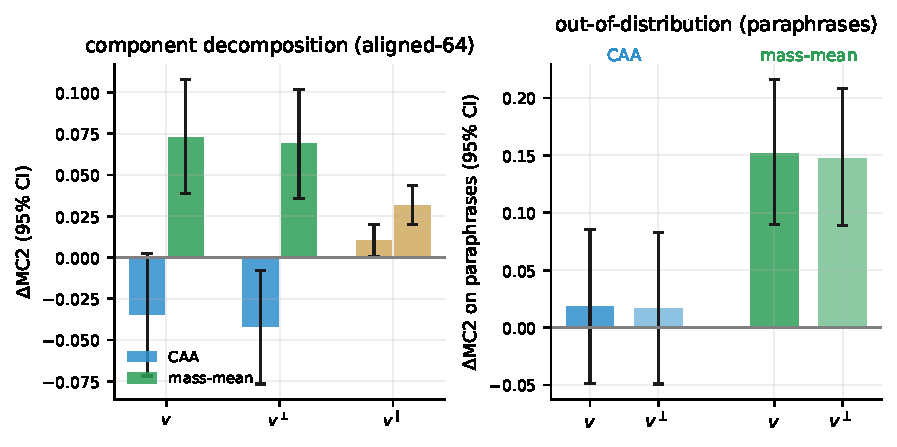
\includegraphics[width=0.95\textwidth]{../figures/decomposition.pdf}
\caption{Left: $\Delta$MC2 of the unprojected vector $v$, its orthogonal projection $\vperp$, and its readout-aligned parallel component $\vpar$ (aligned-64), with 95\% intervals. The projection preserves the mass-mean effect; the parallel component removed by aligned-64 projection delivers less than half of it. Right: the same comparison on model-paraphrased questions.}
\label{fig:decomp}
\end{figure}

\begin{figure}[t]
\centering
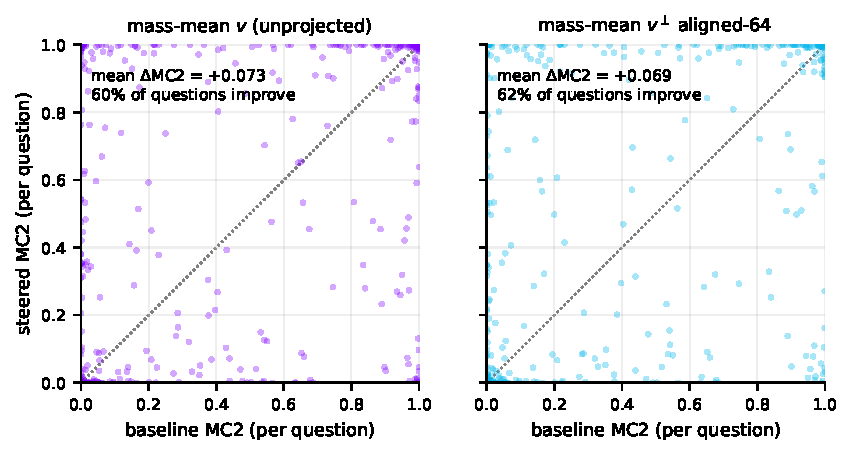
\includegraphics[width=0.92\textwidth]{../figures/scatter_perq.pdf}
\caption{Per-question MC2 under the mass-mean vector (left) and its aligned-64 projection (right), against baseline. The two distributions are nearly identical: the projection preserves the mean effect and its per-question structure.}
\label{fig:scatter}
\end{figure}
\FloatBarrier

\subsection{Curated vocabulary trajectories after aligned-64 projection}\label{sec:lens}

Figure~\ref{fig:lens} compares curated honest-shift trajectories under $v$, aligned-64 $\vperp$, and $\vpar$.

\begin{figure}[h]
\centering
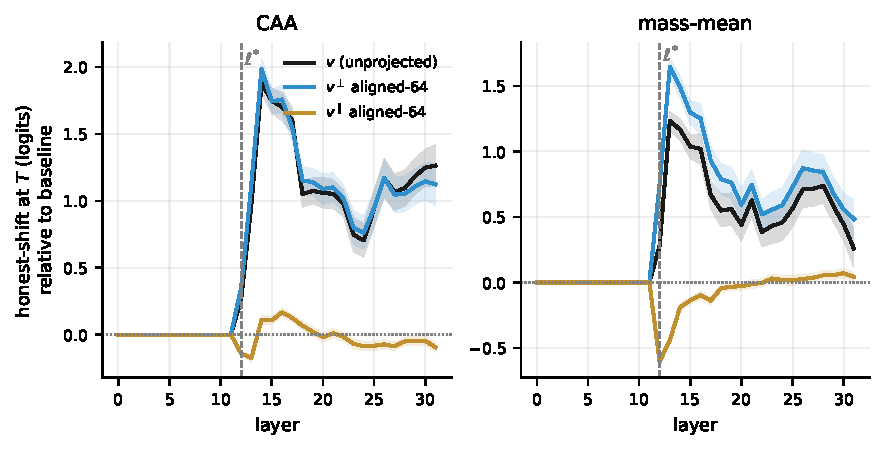
\includegraphics[width=0.95\textwidth]{../figures/lens_resynthesis.pdf}
\caption{Logit-lens trajectories of the curated honest shift by layer for CAA and mass-mean, relative to baseline and evaluated through the model's final norm. The vertical dashed line marks the injection layer. Curves show $v$, aligned-64 $\vperp$, and the removed component $\vpar$.}
\label{fig:lens}
\end{figure}
\FloatBarrier

After injection, each $\vperp$ follows its corresponding unprojected trajectory: it tracks CAA's and exceeds mass-mean's. The removed component $\vpar$ produces no sustained shift. The trajectories therefore show that aligned-64 excision leaves the curated honest shift intact. Because the curated tokens are not the excised set, this plot does not by itself identify downstream reconstruction. On the curated readout, the per-prompt ratio is $\rho_\eta = \DecEtaCurRho$ \DecEtaCurRhoCI{} for CAA (baseline word-shift \DecEtaCurDeltaVdec{} logits) and $\MmEtaCurRho$ \MmEtaCurRhoCI{} for mass-mean (\MmEtaCurDeltaVdec{} logits). The mass-mean projection exceeds the original word-level shift because the excised component pushed against the curated contrast, as shown by $\vpar$'s negative deflection at $\ell^{*}$ in Figure~\ref{fig:lens}.

The spillover lexicon tests synonyms that share no word stem with any projected set. It gives $\rho_\eta = \DecEtaSpillRho$ for CAA (word-shift \DecEtaSpillDeltaVdec{} logits) and $\MmEtaSpillRho$ for mass-mean (word-shift \MmEtaSpillDeltaVdec{} logits). The latter is a small depression of the spillover contrast that projection preserves. Similar shifts therefore also appear on unprojected synonyms. Because single-token filtering leaves only two deceptive surface forms, these ratios are supporting evidence rather than a separate generalization claim.

\subsection{Free-generation results match the multiple-choice pattern}\label{sec:freegen}

Because teacher-forced multiple choice can miss generation collapse (Section~\ref{sec:broken}), we also generate free-form answers to \FreeGenN{} test questions. The \emph{unsteered} model judges each answer using the question and reference correct and incorrect answers. Steering is active during generation but not judging.

Baseline judged truthfulness is \FreeGenBase. CAA lowers it ($\Delta = \DecFreeGenVdecDelta$ \DecFreeGenVdecDeltaCI), while mass-mean raises it ($\Delta = \MmFreeGenVdecDelta$ \MmFreeGenVdecDeltaCI). The aligned-64 projection $\vperp$ retains the mass-mean gain ($\Delta = \MmFreeGenVperpDelta$ \MmFreeGenVperpDeltaCI), matching the multiple-choice result. Unlike teacher-forced scoring, this endpoint depends on the model's own continuation, so it checks that the projected gain survives in usable generation. The judge is the unsteered base model rather than a human or independent model, so this result is corroborative.

The remaining question is whether this separation between effect existence and effect depth survives a change of model.
